\chapter{列举环境和算法环境}
以下资料来自宏包说明和网络,翻译不一定正确:

在LaTeX中有三种基本的列举(列表)环境,即enumerate(编号)、itemize(分条目)和description(描述)环境。调整latex的列表环境时,使用 enumitem 宏包可以方便的调整间距(注意区分包名和环境名)和自定义编号样式。

\section{调整间距}
三种基本环境无论哪一种,间距的调整都是一样的。调整间距的参数命令包括两类:垂直间距和水平间距。各种距离的定义如图\ref{enumitem}所示。下图的来源一直找不到,可能是旧版本的宏包说明,新版已经删掉了下面的注释了。
\begin{figure}[htbp]
	\centering
	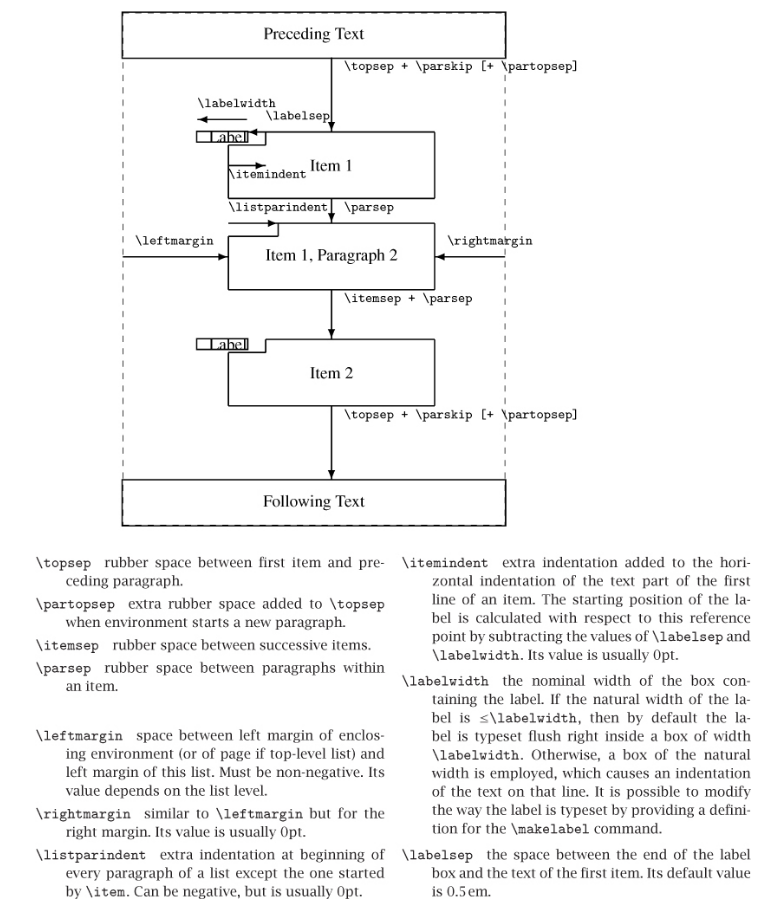
\includegraphics[scale=0.6]{Fig/enumitem1.png}
	\caption{\label{enumitem}enumitem包对各种间距的定义}
\end{figure}

现先总结出所推荐的间距设置,无编号的:
\begin{lstlisting}
\begin{itemize}[topsep = 0 pt, itemsep= 0 pt, parsep=0pt, partopsep=0pt, leftmargin=36pt, itemindent=0pt, labelsep=6pt, listparindent=24pt]
	\item 第一项。内容内容内容内容内容内容内容内容内容内容内容内容内容内容内容内容内容内容内容内容内容内容内容内容内容内容内容内容内容内容

	\item 第二项。内容内容内容内容内容内容内容内容内容内容内容内容内容内容内容内容内容内容内容内容内容内容内容内容内容内容内容内容内容内容
	
\end{itemize}
\end{lstlisting}
效果:
\begin{itemize}[topsep = 0 pt, itemsep= 0 pt, parsep=0pt, partopsep=0pt, leftmargin=36pt, itemindent=0pt, labelsep=6pt, listparindent=24pt]
	\item 第一项。内容内容内容内容内容内容内容内容内容内容内容内容内容内容内容内容内容内容内容内容内容内容内容内容内容内容内容内容内容内容

	\item 第二项。内容内容内容内容内容内容内容内容内容内容内容内容内容内容内容内容内容内容内容内容内容内容内容内容内容内容内容内容内容内容
	
\end{itemize}

有编号的:
\begin{lstlisting}
\begin{enumerate}[topsep = 0 pt, itemsep= 0 pt, parsep=0pt, partopsep=0pt, leftmargin=44pt, itemindent=0pt, labelsep=6pt, label=(\arabic*)]
	\item 第一项。内容内容内容内容内容内容内容内容内容内容内容内容内容内容内容内容内容内容内容内容内容内容内容内容内容内容内容内容内容内容

	\item 第二项。内容内容内容内容内容内容内容内容内容内容内容内容内容内容内容内容内容内容内容内容内容内容内容内容内容内容内容内容内容内容
	
\end{enumerate}
\end{lstlisting}
效果:
\begin{enumerate}[topsep = 0 pt, itemsep= 0 pt, parsep=0pt, partopsep=0pt, leftmargin=44pt, itemindent=0pt, labelsep=6pt, label=(\arabic*)]
	\item 第一项。内容内容内容内容内容内容内容内容内容内容内容内容内容内容内容内容内容内容内容内容内容内容内容内容内容内容内容内容内容内容

	\item 第二项。内容内容内容内容内容内容内容内容内容内容内容内容内容内容内容内容内容内容内容内容内容内容内容内容内容内容内容内容内容内容
	
\end{enumerate}

下面两节分别讨论参数设置规则。
\subsection{垂直间距}
摘抄宏包说明:
\begin{itemize}[topsep = 0 pt, itemsep= 0 pt, parsep=0pt, partopsep=0pt, leftmargin=36pt, itemindent=0pt, labelsep=6pt, listparindent=24pt]
	\item topsep控制列表环境与上文之间的距离。第一项和前一段之间的空间。

	\item itemsep 条目之间的距离

	\item parsep 条目里面段落之间的距离
 
	\item partopsep 条目与下面段落的距离。当环境开始一个新段落时,额外的空间被添加到 \textbackslash{}topsep。
\end{itemize}

论文中希望上述距离都为0pt,如:
\begin{lstlisting}
	\begin{itemize}[topsep = 0 pt, itemsep= 0 pt, parsep=0pt, partopsep=0pt]
		\item 第一项。
		\item 第二项
		\item 第三项。
	\end{itemize}
\end{lstlisting}
效果为:
\begin{itemize}[topsep = 0 pt, itemsep= 0 pt, parsep=0pt, partopsep=0pt]
	\item 第一项。
	\item 第二项
	\item 第三项。
\end{itemize}


\subsection{水平间距}
% 正文12pt
水平间距调整比较复杂,对照宏包说明给出的图,下面内容参考了宏包原文和网络资料:
\begin{itemize}[topsep = 0 pt, itemsep= 0 pt, parsep=0pt, partopsep=0pt, leftmargin=36pt, itemindent=0pt, labelsep=6pt, listparindent=24pt]
	\item 为页面的左边距)和该列表的左边距之间的空间。 必须是非负数。 它的值取决于表,则为页面的左边距)和该列表的左边距之间的空间。 必须是非负数。 它的值取决于列表级别。
	\item rightmargin       列表环境右边的空白长度。类似于 \textbackslash{}leftmargin 但用于右边距。 它的值通常是 0pt。
	\item labelsep       标号与列表第一项文本左侧的距离。标签框的末尾和第一项的文本之间的空间。 它的默认值为 0.5 em。
	\item itemindent       条目的缩进距离。添加到项目第一行文本部分的水平缩进的额外缩进。 通过减去 labelsep 和 labelwidth 的值,相对于该参考点计算标签的起始位置。 它的值通常是 0pt。注:理解这个变量时,查看图\ref{enumitem}的顺序应该按照箭头从左到右,先leftmargin再itemindent,然后再labelsep,最后labelwidth。即箭头的起始点是基准点。若itemindent=0pt,则leftmargin-labelsep-编号长度的结果就是编号起始位置。
	\item labelwidth       包含标签的框的标称宽度。 如果标签的自然宽度为 < labelwidth,则默认情况下,标签在宽度为 (labelwidth) 的框内右对齐排版。否则,使用自然宽度的框,这会导致该行上的文本缩进。 可以通过为 \textbackslash{}makelabel 命令提供定义来修改标签的排版方式。
	\item listparindent       条目下面段落的缩进距离。除了以 litem 开头的段落之外,列表的每个段落的开头都有额外的缩进。 可以为负数,但通常为 0pt。
\end{itemize}

无编号的水平间距,给出两张方案
 
第一种:
\begin{itemize}[topsep = 0 pt, itemsep= 0 pt, parsep=0pt, partopsep=0pt, leftmargin=36pt, itemindent=0pt, labelsep=6pt, listparindent=24pt]
	\item 第一项。内容内容内容内容内容内容内容内容内容内容内容内容内容内容内容内容内容内容内容内容内容内容内容内容内容内容内容内容内容内容

	% 第一项的第二段。内容内容内容内容内容内容内容内容内容内容内容内容内容内容内容内容内容内容内容内容内容内容内容内容内容内容内容内容内容内容
	\item 第二项。内容内容内容内容内容内容内容内容内容内容内容内容内容内容内容内容内容内容内容内容内容内容内容内容内容内容内容内容内容内容
	
\end{itemize}


第二种:
\begin{itemize}[topsep = 0 pt, itemsep= 0 pt, parsep=0pt, partopsep=0pt, leftmargin=0pt, itemindent=36pt, labelsep=6pt, listparindent=24pt]
	\item 第一项。内容内容内容内容内容内容内容内容内容内容内容内容内容内容内容内容内容内容内容内容内容内容内容内容内容内容内容内容内容内容

	% 第一项的第二段。内容内容内容内容内容内容内容内容内容内容内容内容内容内容内容内容内容内容内容内容内容内容内容内容内容内容内容内容内容内容
	\item 第二项。内容内容内容内容内容内容内容内容内容内容内容内容内容内容内容内容内容内容内容内容内容内容内容内容内容内容内容内容内容内容
	
\end{itemize}

推荐第一种。

有编号的水平间距,下面给出三种方案:
注:labelsep是某一项文字和编号框的距离,一般就设为一个空格6pt,要使编号左侧缩进两格,itemindent-labelsep要等于编号长度。注意编号是右对齐,向左扩展的。

第一种方案是整体右移两格,文字距离编号一个空格,然后第二行文字和第一行对齐:
\begin{enumerate}[topsep = 0 pt, itemsep= 0 pt, parsep=0pt, partopsep=0pt, leftmargin=44pt, itemindent=0pt, labelsep=6pt, label=(\arabic*)]
	\item 第一项。内容内容内容内容内容内容内容内容内容内容内容内容内容内容内容内容内容内容内容内容内容内容内容内容内容内容内容内容内容内容

	% 第一项的第二段。内容内容内容内容内容内容内容内容内容内容内容内容内容内容内容内容内容内容内容内容内容内容内容内容内容内容内容内容内容内容
	\item 第二项。内容内容内容内容内容内容内容内容内容内容内容内容内容内容内容内容内容内容内容内容内容内容内容内容内容内容内容内容内容内容
	
\end{enumerate}

第二种方案是和论文撰写规范的格式一样,注意不是论文撰写规范规定的格式,规范里没有规定这些格式。如:
\begin{enumerate}[topsep = 0 pt, itemsep= 0 pt, parsep=0pt, partopsep=0pt, leftmargin=0pt, itemindent=44pt, labelsep=6pt, listparindent=24pt, label=(\arabic*)]
	\item 第一项。内容内容内容内容内容内容内容内容内容内容内容内容内容内容内容内容内容内容内容内容内容内容内容内容内容内容内容内容内容内容

	% 第一项的第二段。内容内容内容内容内容内容内容内容内容内容内容内容内容内容内容内容内容内容内容内容内容内容内容内容内容内容内容内容内容内容
	\item 第二项。内容内容内容内容内容内容内容内容内容内容内容内容内容内容内容内容内容内容内容内容内容内容内容内容内容内容内容内容内容内容
	
\end{enumerate}

第三种方案是整体右移两格,文字距离编号一个空格,第二行文字不再右移:
\begin{enumerate}[topsep = 0 pt, itemsep= 0 pt, parsep=0pt, partopsep=0pt, leftmargin=24pt, itemindent=20pt, labelsep=6pt, listparindent=20pt, label=(\arabic*)]
	\item 第一项。内容内容内容内容内容内容内容内容内容内容内容内容内容内容内容内容内容内容内容内容内容内容内容内容内容内容内容内容内容内容

	% 第一项的第二段。内容内容内容内容内容内容内容内容内容内容内容内容内容内容内容内容内容内容内容内容内容内容内容内容内容内容内容内容内容内容
	\item 第二项。内容内容内容内容内容内容内容内容内容内容内容内容内容内容内容内容内容内容内容内容内容内容内容内容内容内容内容内容内容内容
	
\end{enumerate}

推荐第一种。

\section{enumerate标签样式}
除上述小括号数字的编号方法外,还有斜体字母等。在使用enumerate的时候,label的问题就是使用计数的字符,是阿拉伯数字、罗马、中文、还是希腊字符的问题。

\subsection{小括号阿拉伯数字}
% 小括号阿拉伯数字,用 label=\arabic*)
\begin{enumerate}[topsep = 0 pt, itemsep= 0 pt, parsep=0pt, partopsep=0pt, leftmargin=0pt, itemindent=44pt, labelsep=6pt, listparindent=24pt, label=\arabic*)]
	\item 第一项。

	% 第一项的第二段。
	\item 第二项
	
	% 第二项的第二段。
	\item 第三项。
	
	% 第三项的第二段。
\end{enumerate}



\subsection{斜体字母}
% 斜体字母,用 label=\emph{\alph*}
\begin{enumerate}[topsep = 0 pt, itemsep= 0 pt, parsep=0pt, partopsep=0pt, leftmargin=0pt, itemindent=44pt, labelsep=6pt, listparindent=24pt, label=\emph{\alph*}.]
	\item 第一项。

	% 第一项的第二段。
	\item 第二项
	
	% 第二项的第二段。
	\item 第三项。
	
	% 第三项的第二段。
\end{enumerate}

\subsection{大写罗马字母}
% 大写罗马字母,用 label=(\Roman*)
\begin{enumerate}[topsep = 0 pt, itemsep= 0 pt, parsep=0pt, partopsep=0pt, leftmargin=0pt, itemindent=44pt, labelsep=6pt, listparindent=24pt, label=(\Roman*)]
	\item 第一项。

	% 第一项的第二段。
	\item 第二项
	
	% 第二项的第二段。
	\item 第三项。
	
	% 第三项的第二段。
\end{enumerate}

\section{算法环境}
算法环境原来的模板就有,用户可以按需使用,后来实验室有同学写的我看不错,就更新了一下(.cls文件算法环境部份)。

以下资料来自往届毕业生:
\begin{algorithm}
    \caption{RemoveRedundantNodes}
    \label{冗余节点删除策略}
    \begin{algorithmic}[1]
        \setlength{\baselineskip}{16pt} % 设置伪代码行间距
            \State  $\textbf{Input:}\text{ initPath}$
            \State  $\text{optiPath} \gets \text{initPath};$
            \State  $\text{index} \gets 1;$
            \While{$\text{index} <= \text{optiPath.size()}$-2}
                \If{$\text{ObstacleFree}(\text{optiPath[index]},\text{optiPath[index+2]})$}
                    \State $\text{optiPath} \gets \text{optiPath.remove}(\text{index+1});$
                \Else
                    \State $\text{index} \gets \text{index} + 1;$
                \EndIf
            \EndWhile
            \State $\textbf{Output:}\text{ optiPath}$
\end{algorithmic}
\end{algorithm}


\begin{algorithm}
    \caption{RRT-Connect算法}
    \label{RRT-Connect算法}
    \begin{algorithmic}[1]
        \setlength{\baselineskip}{16pt}
        \State $\boldsymbol{T}_1\leftarrow\boldsymbol{x}_{start};\boldsymbol{E}_1\leftarrow\emptyset;$
        \State $\boldsymbol{T}_2\leftarrow\boldsymbol{x}_{end};\boldsymbol{E}_2\leftarrow\emptyset;$
        \State $\text{Final} \gets false ;$
        \While{$not$ Final}
            \State $\boldsymbol{x}_{rand}\gets\text{RandomSample}();$
            \State $\boldsymbol{x}_{near1}\gets\text{GetNearest}(\boldsymbol{x}_{rand},\boldsymbol{T}_1);$
            \State $\boldsymbol{x}_{new1}\gets\text{GetNewNode}(\boldsymbol{x}_{rand},\boldsymbol{x}_{near1},step);$
            \If{$\text{ObstacleFree}(\boldsymbol{x}_{new1},\boldsymbol{x}_{near1})$}
                \State $\boldsymbol{T}_1\leftarrow \boldsymbol{T}_1\cup\{\boldsymbol{x}_{new1}\};$
                $\boldsymbol{E}_1\leftarrow \boldsymbol{E}_1\cup\{\boldsymbol{x}_{near1},\boldsymbol{x}_{new1}\};$
                \State $\boldsymbol{x}_{near2}\gets\text{GetNearest}(\boldsymbol{x}_{new1},\boldsymbol{T}_2);$
                \State $\boldsymbol{x}_{new2}\gets\text{GetNewNode}(\boldsymbol{x}_{new1},\boldsymbol{x}_{near2},step);$
                \While{$\text{ObstacleFree}(\boldsymbol{x}_{new2},\boldsymbol{x}_{near2})$}
                \State $\boldsymbol{T}_2\leftarrow \boldsymbol{T}_2\cup\{\boldsymbol{x}_{new2}\};$
                $\boldsymbol{E}_2\leftarrow \boldsymbol{E}_2\cup\{\boldsymbol{x}_{near2},\boldsymbol{x}_{new2}\};$
                \State $\boldsymbol{x}_{near\_tmp}\gets\text{GetNearest}(\boldsymbol{x}_{new2},\boldsymbol{T}_1);$
                \If{$\text{ObstacleFree}(\boldsymbol{x}_{new2},\boldsymbol{x}_{near\_tmp}) \text{ }and \text{ dist}(\boldsymbol{x}_{new2},\boldsymbol{x}_{near\_tmp}) < d_{th}$}
                    \State $\text{Final} \gets true ;$
                    \State break;
                \EndIf
                \State $\boldsymbol{x}_{near2}\gets\boldsymbol{x}_{new2};$
                \State $\boldsymbol{x}_{new2}\gets\text{GetNewNode}(\boldsymbol{x}_{new1},\boldsymbol{x}_{near2},step);$
                \EndWhile
                \State swap$(\boldsymbol{T}_1,\boldsymbol{T}_2);$swap$(\boldsymbol{E}_1,\boldsymbol{E}_2);$
            \EndIf
        \EndWhile \\
        \Return $(\boldsymbol{T}_1,\boldsymbol{T}_2,\boldsymbol{E}_1,\boldsymbol{E}_2)$
\end{algorithmic}
\end{algorithm}